\subsection{Example}

Let us present a solution for the problem stated in motivating example section (\ref{motivExample}): grammar $G_1$ is a query and we want to find all paths in graph $M$ (presented in picture~\ref{input}) which match this query.
Result SPPF for this input is presented in figure~\ref{SPPF}. Note that presented version does not contains redundant nodes.
Each terminal node corresponds to the edge in the input graph: for each node with label $(v_0, T, v_1)$ there is $e\in E: e=(v_0,T,v_1)$.
We duplicate terminal nodes only for figure simplification.

\begin{figure}[h]
    \begin{center}
        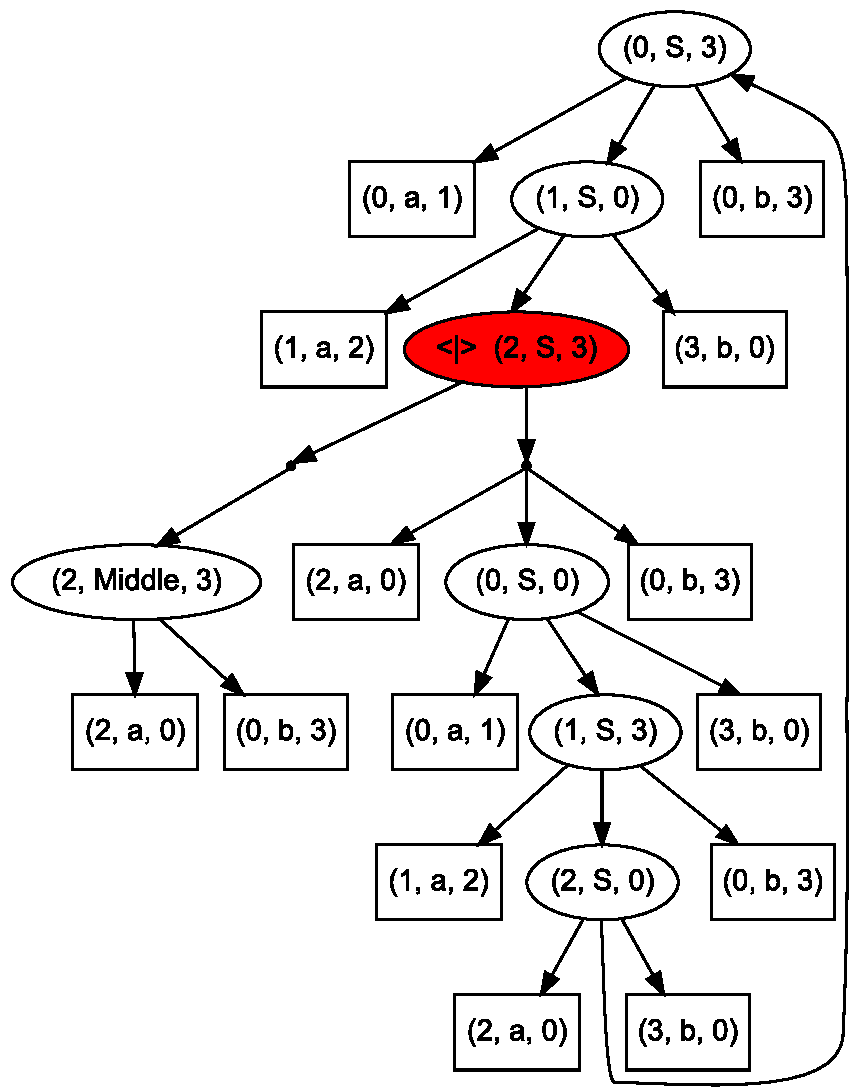
\includegraphics[width=8cm]{dot/AnBn.pdf}
        \caption{Result SPPF for input graph $M$(fig.~\ref{input}) and query $G_1$(fig.~\ref{grammarG})}
        \label{SPPF}        
    \end{center}
\end{figure}

    
As an example of derivation structure usage, we can find a middle of any path in example simply by finding correspondent nonterminal \textit{Middle} in SPPF.
So we can find out that there is only one (common) middle for all results, and it is a vertex with $id = 0$. 

Extensions stored in nodes allow us to check whether path from $u$ to $v$ exists and to extract it. 
We need only to traverse SPPF which can be done in polynomial time (in terms of SPPF size) to extract any path . 

Lets find paths $p_i$ such that $S {\xRightarrow[G_1]{}}^{*} \Omega(p_i)$ and $p_i$ starts from the vertex $0$.
To do this, we should find vertices with label $(0, S, \_)$ in SPPF.
(There are two vertices with such labels: $(0, S, 0)$ and $(0, S, 3)$.)
Then let us to extract corresponded paths from SPPF.
There is a cycle in SPPF in our example, so there are \textbf{at least} two different paths: $$p_0=\{(0,a,1);(1,a,2);(2,a,0);(0,b,3);(3,b,0);(0,b,3)\}$$ and 
\begin{align*}
p_1=\{&(0,a,1);(1,a,2);(2,a,0);(0,a,1);(1,a,2);(2,a,0);\\ &(0,b,3);(3,b,0);(0,b,3);(3,b,0);(0,b,3);(3,b,0)\}.
\end{align*}


We demonstrate that SPPF which was constructed by described algorithm can be useful for query result investigation. 
But in some cases explicit representation of matched subgraph is preferable, and required subgraph may be extracted from SPPF trivially by its traversal.
